
\documentclass{abgabe}
\begin{document}

\begin{questions}
    \qformat{\thequestion. \textbf{\thequestiontitle} \hfill}
    \titledquestion{Aktivitätsdiagramm Fahrkartenautomat}

    In \href{https://www.ili.fh-aachen.de/ilias.php?ref_id=813760&obj_id=206096&obj_type=PageObject&cmd=layout&cmdClass=illmpresentationgui&cmdNode=gh&baseClass=ilLMPresentationGUI}{Übung 3} wurde ein Lastenheft für einen Fahrkartenautomaten erstellt.

    \begin{parts}
        \part
        Dokumentieren Sie den Anwendungsfall „Fahrkarte kaufen“ mit Hilfe eines UML-Aktivitätsdiagrammes, das z.B. mit \href{https://www.ili.fh-aachen.de/ilias.php?baseClass=ilLinkResourceHandlerGUI&ref_id=341847&cmd=calldirectlink}{Visual Paradigm} erstellt wird.

        Teilen Sie das Aktivitätsdiagramm dabei in die folgenden Partitionen (Schwimmbahnen) auf:
        \begin{itemize}
            \item Kunde: Interaktion des Kunden mit dem Automaten
            \item Display: Anzeige von Text
            \item Automat: Eingaben einlesen, Rückgeldberechnung, Kartendruck, \ldots
        \end{itemize}
        Modellieren Sie dabei Geld und Fahrkarten als Objektknoten!

        \emph{Hinweise:}
        \begin{itemize}
            \item Der Automat arbeitet nur mit Bargeld.
            \item Beachten Sie, dass der Bezahlvorgang auch abgebrochen werden kann.
            \item Verwenden Sie Parallelitäten, wo es für Sie Sinn ergibt.
            \item Beachten Sie auch den Fall, wenn der Automat nicht genug Rückgeld geben kann.
        \end{itemize}

        \newpage
        \begin{solution}
            \begin{center}
                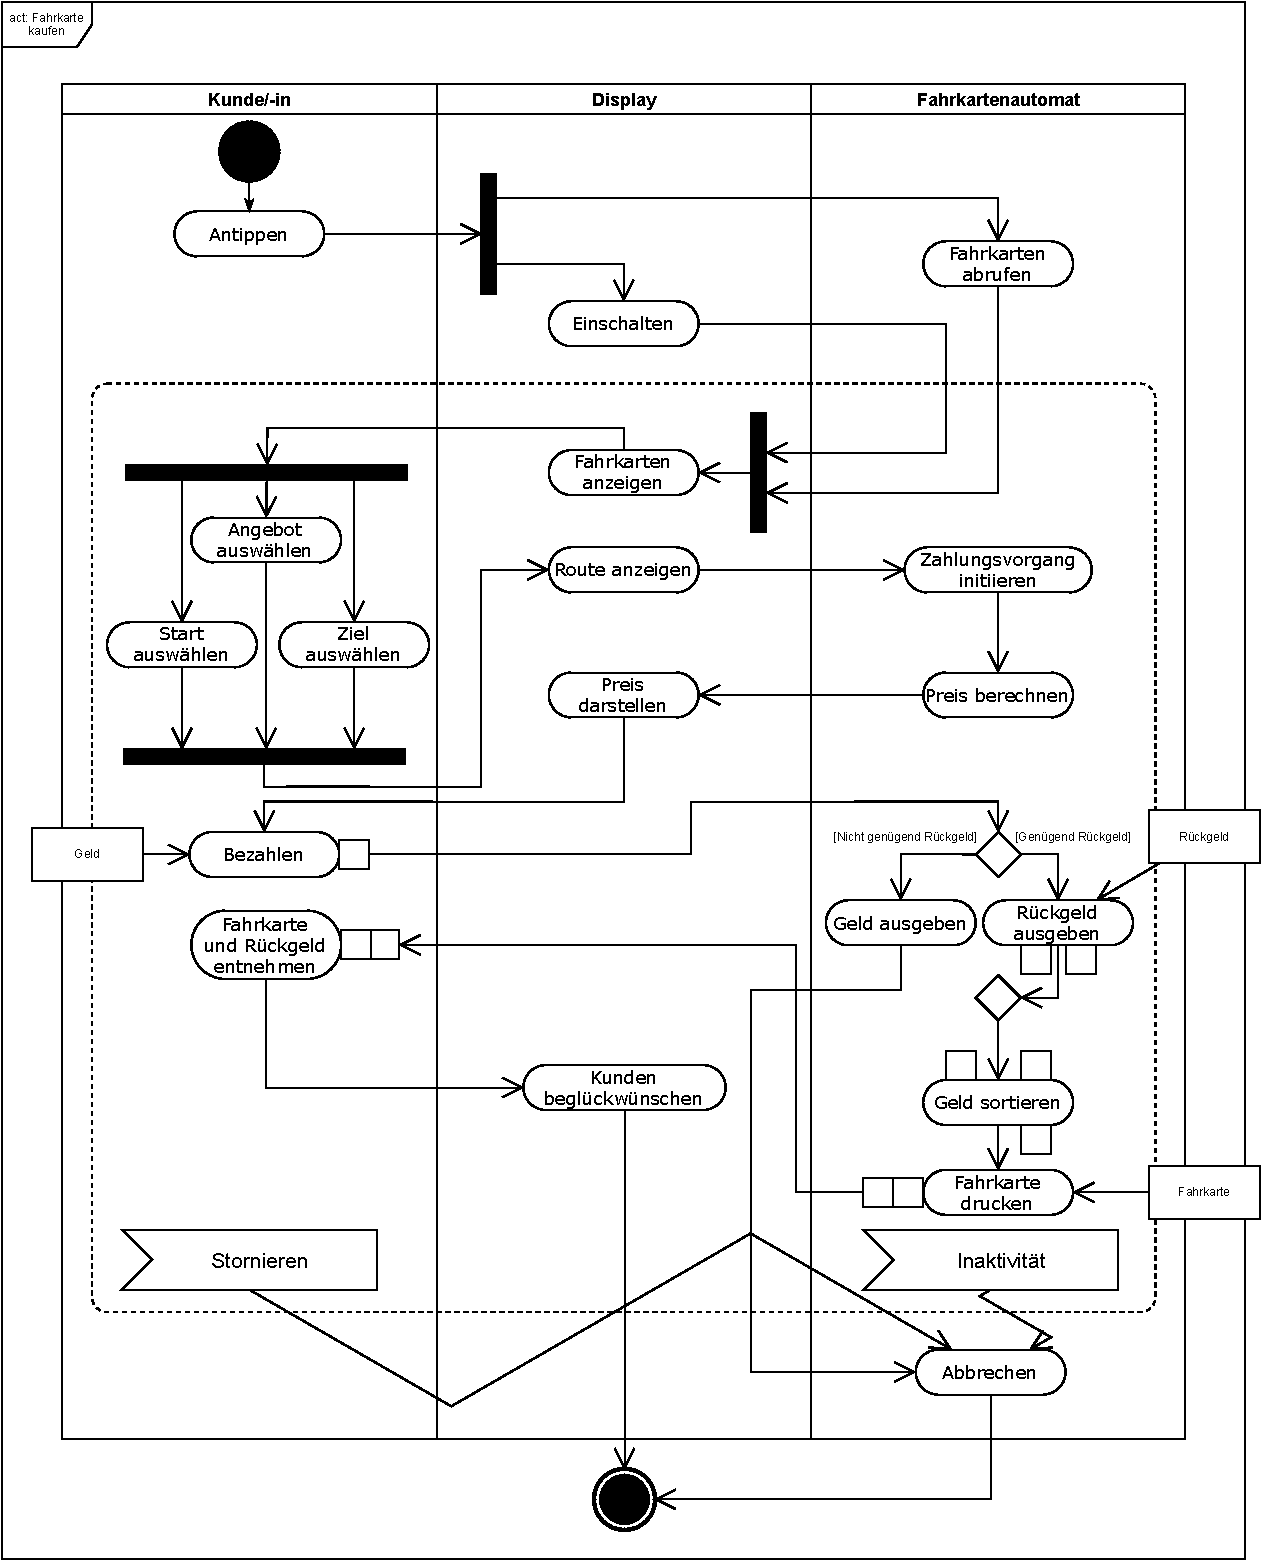
\includegraphics[width=\textwidth]{swt_h04_activity.pdf}
            \end{center}
        \end{solution}

        \newpage
        \part
        Beschreiben Sie mit eigenen Worten, wie der Zusammenhang zwischen UML-Use-Case-Diagrammen, speziell der Szenariobeschreibung, und den UML-Aktivitätsdiagrammen ist.
        \begin{solution}
            StackOverflow-User \href{https://stackoverflow.com/a/62550230/9055591}{Christophe} fasst es sehr gut zusammen:
            \begin{displayquote}
                \textelp{}

                \begin{itemize}
                    \item Use-case diagrams are about what the systems has to offer to fulfil the requirements.
                          Each use-case correspond to a \emph{set of behaviors} that may be performed in interaction with the actors for helping them achieving their goals.
                    \item The activity diagram is about how the system performs \emph{elementary behaviors}, or more complex \emph{sets of behaviors}
                \end{itemize}
                Use-case isn't about the internals of the system.
                It's about its purpose and main relation with the outside world.
                There is absolutely no sequential order between the use-cases shown in such diagram.
                A user may read it and get an answer to the question \enquote{what's in for me?}.

                Activity is on contrary not about the outside world and not about actors.
                It's about the internals of the system:
                its internal flows, which follow an order that can be deduced from the control and dataflow semantics.
                A developer may read it and get an answer to the question \enquote{How shall this work?}

                \textelp{}

                In conclusion, there is not necessarily a direct mapping between activity and use-cases, since they represent different realities.
                However, if such a mapping exist, it's at least one activity diagram per use-case (bubble).
            \end{displayquote}
        \end{solution}
    \end{parts}

\end{questions}
\end{document}